% This is based on the LLNCS.DEM the demonstration file of
% the LaTeX macro package from Springer-Verlag
% for Lecture Notes in Computer Science,
% version 2.4 for LaTeX2e as of 16. April 2010
%
% See http://www.springer.com/computer/lncs/lncs+authors?SGWID=0-40209-0-0-0
% for the full guidelines.
%

\documentclass{llncs}

\usepackage[utf8]{inputenc}
\usepackage[T1]{fontenc}
\usepackage[polish]{babel}
\usepackage[colorinlistoftodos]{todonotes}
\usepackage{hyperref}
\usepackage{float}
\usepackage{graphicx}
\usepackage{caption}
\usepackage{subcaption}


\begin{document}

\title{Ewolucyjna konstrukcja modeli neuronowych}
%
\titlerunning{ConvConnect4}  % abbreviated title (for running head)
%                                     also used for the TOC unless
%                                     \toctitle is used
%
\author{Tomasz Janiszewski\inst{1} \and Jakub Dutkowski\inst{2}}
%
\authorrunning{Tomasz Janiszewski, Jakub Dutkowski} % abbreviated author list (for running head)
%
%%%% list of authors for the TOC (use if author list has to be modified)
\tocauthor{Tomasz Janiszewski and Jakub Dutkowski}

\institute{Politechnika Warszawska\\
Wydział Matematyki i Nauk Informacyjnych
\email{janiszewskit@student.mini.pw.edu.pl}~~
\email{dutkowskij@student.mini.pw.edu.pl}}

\maketitle              % typeset the title of the contribution

\keywords{Connect4, Neural Network, Evolutionary Algorithm, Neuroevolution, Connect Four}
%
\section{Zadanie}
Zbadać efektywność zastosowania programowania genetycznego do konstrukcji neuronowych sieci MLP 
(perceptronów wielowarstwowych) z pojedynczą warstwą ukrytą.
Eksperymenty oprzeć na wybranym zestawie zadań regresji.

\section{Specyfikacja wstępna}

\subsection{Wstęp}
Celem projektu jest zbadanie przydatności programowania genetycznego do konstrukcji neuronowych sieci MLP.
W projekcie skupimy się na budowaniu sieci grającej w Connect Four (\emph{pol. Czwórki}) \cite{connect4:wiki}
na planszy o rozmiarze $4 \times 4$.

\subsection{Opis problemu}
Podczas konstrukcji sieci neuronowych istnieje problem doboru parametrów tej sieci takich jak:
\begin{itemize}
	\item liczba warstw ukrytych
	\item liczba neuronów w każdej warstwie
	\item funkcja aktywacji neuronu
	\item obecność biasu
	\item wagi początkowe
	\item współczynniki nauki
\end{itemize}
aby proces uczenia był jak najbardziej efektywny. Algorytmy oparte na metodzie propagacji wstecznej osiągają
dość dobre rezultaty, jednak nie są odporne na utykanie w ekstremach lokalnych oraz osiągają małą zbieżność
na płaskich odcinkach funkcji celu. Aby wyeliminować te problemy stosuje się takie techniki jak symulowane wyżarzanie.
W niniejszej pracy chcemy się zająć użyciem algorytmu ewolucyjnego aby znaleźć optymalną strukturę sieci
dla danego problemu przeszukując jak najmniejszy obszar.

\subsection{Sieć neuronowa}
Badana rodzina sieci neuronowych będzie grała w Connect Four na planszy o rozmiarze $4 \times 4$. Plansza będzie zakodowana
jako tablica szesnastu ($16$) elementów, z których każdy może przyjmować wartości $-1,0,1$ oznaczające
\begin{itemize}
	\item[$-1$] pole zajęte przez przeciwnika
	\item[$0$] pole wolne
	\item[$1$] pole zajęte przez gracza aktywnego
\end{itemize}
Na wyjściu sieci dla zadanej planszy znajduje się liczba oznaczająca ruch dla danego na wejściu stanu planszy.

\subsection{Algorytm uczenia}
Sieć będzie uczona za pomocą algorytmu propagacji wstecznej. Dane treningowe wygenerowane zostaną za pomocą programu
opartego o algorytm alfa-beta.

\subsection{Algorytm ewolucyjny}
W projekcie zastosujemy klasyczny algorytm genetyczny.
\subsubsection{Fenotyp}
\begin{itemize}
	\item funkcja aktywacji
	\item liczba neuronów w warstwie ukrytej
	\item wektor wag
\end{itemize}

\subsubsection{Genotyp}
\begin{itemize}
	\item funkcja aktywacji -- 3 elementowy wektor binarny określający funkcje aktywacji
	\item liczba neuronów w warstwie ukrytej -- dodatnia liczba całkowita
	\item wektor wag -- dodatnia liczba całkowita określająca ziarno losowania wektora wag
	\item bias -- 3 elementowy wektor binarny okręslający obecność biasu dla poszczególnych warstw
\end{itemize}

\begin{example}

\begin{tabular}{ | c | c | c | c | c | c | c | c | }
	\hline
	0 & 1 & 0 & 5 & 2356 & 0 & 1 & 1\\
	\hline
\end{tabular}
\\
Powyższa definicja oznacza sieć neuronową złożoną z 3 warstw 
(wejście -- 4 neurony, warstwa ukryta -- 5, wyjście -- 1).
Warstwa wejściowa i wyjściowa korzystają z tangensa hiperbolicznego jako funkcji przejścia natomiast 
warstwa ukryta używa funkcji sigmoidalnej. Bias jest obecny w drugiej i trzeciej warstwie. Ziarno
generatora liczb losowych ustawione jest na $2356$.
\end{example}

\subsubsection{Krzyżowanie}
Krzyżowanie funkcji aktywacji i biasu oparte będzie na krzyżowaniu dwupunktowym. Natomiast
krzyżowanie liczby neuronów w warstwie ukrytej i wektora wag na krzyżowaniu uśredniającym.

\subsubsection{Mutacje}
Mutacja funkcji przejścia i biasu będzie polegała na zamianie bitu na losowy.
Mutacja liczby neuronów w warstwie ukrytej i wektora wag będzie polegało na zmianie
wartości o losowy współczynnik.

\subsubsection{Funkcja przystosowania}
Wartością funkcji przystosowania będzie błąd na zbiorze testowym po ustalonym treningu.

\subsubsection{Metoda selekcji}
Do selekcji zostanie użyta metoda ruletki.

\section{Sprawozdanie}

Z uwagi na długi czas nauki perceptronu przy prototypie wykorzystano perceptron aproksymujący funkcję
$f(x) = x^{1/2}$, uczony zbiorem $\Omega (\overline{\Omega} = 10)$.

Na podstawie doświadczeń z prototypem podjęto decyzję o następujących istotnych zmianach w stosunku do specyfikacji.

\subsection{Istotne zmiany w stosunku do specyfikacji}
\subsubsection{Algorytm uczenia}
Z uwagi na wolną zbieżność i konieczność definiowania ścisłych współcznynników nauki w algorytmie propagacji wstecznej
zdecydowano się na użycie algorytmu \texttt{rprop+}\cite{Riedmiller93adirect}
\subsubsection{Genotyp}
Orginalny fenotyp był dość rozbudowany. Zmiany w pojedynczym elemencie często powodowały katastrofalne skutki.
W szczególności element odpowiedzialny za losowy dobór wag zachowywał się w sposób losowy, jego małe zmiany
często oznaczały gigantyczne zmiany w wynikach ewaluacji. W ostatecznej wersji zamieniono ten element na 
wartość skalującą raz ustalony wektor wag.
Z uwagi na łatwość implementacji zdecydowano się na użycie binarnej reprezentacji fenotypu. 
Ponadto zrezygnowano z opcjonalności stosowania \emph{bias} gdyż jego brak zazwyczaj
powoduje wydłużenie procesu uczenia.
\begin{itemize}
	\item funkcja aktywacji -- 3 elementowy wektor binarny określający funkcję aktywacji. Jeśli pierwszy (1) i 
	drugi (2) element są równe to używana jest \emph{tangens hiperboliczny} w przeciwnym wypadku funkcja \emph{sigmoidalna}.
	Trzeci element opowiada za stosowanie bądź nie liniowej transformacji na wyjściu.
	\item liczba neuronów w warstwie ukrytej -- dodatnia liczba całkowita
	\item wektor wag -- dodatnia liczba całkowita określająca skalowanie wylosowanego wektora wag.
	Ustalony wektor wag jest dzielony przez tę liczbę.
\end{itemize}

\subsubsection{Krzyżowanie}
Zdecydowano się zastosować jedno krzyżowanie dla całego chromosomu i wybrano krzyżowanie
jednopunktowe.

\subsubsection{Mutacje}
Z uwagi na zastosowanie binarnej reprezentacji chromosomu, mutacje dotyczą całego chromosomu 
a nie tylko wybranych części.

\subsubsection{Funkcja przystosowania}
W celu skrócenia czasu eksperymentu, zdecydowano na ustalenie progu, po którym nauka zostanie przerwana.
W związku z tym funkcja przystosowania zwraca wartość, która jest iloczynem
liczby wykonanych iteracji oraz sumarycznego błędu na zbiorze uczącym.

\subsubsection{Metoda selekcji}
Ponieważ w wyniku zmian w chromosomie liczba możliwych kombinacji znacząco spadła, zdecydowano się na 
zastosowanie zbioru elitarnego w liczbie nie większej niż dwadzieścia procent (20\%) z całej populacji.

\subsection{Implementacja}
Całość została zaimplementowana przy użyciu środowiska R. Perceptron zaimplementowany został
z użyciem biblioteki \texttt{neurlanet}\cite{R:neuralnet}, natomiast jako schemat algorytmu genetycznego wykorzystano
\texttt{genalg}\cite{R:genalg}. W celu przyspieszenia działania zastosowano cachowanie dostarczane przez bibliotekę
\texttt{R.cache}\cite{R:cache}

\subsection{Wyniki}
Testy przeprowadzono na następujących danych

\begin{table}[H]
\caption{Konfiguracja testowa}
\label{small}
\centering
\begin{tabular}{|c|c|}
  Type                  & binary chromosome \\
  Population size       & 10 \\
  Number of Generations & 10 \\
  Elitism               & 0.2 \\
  Mutation Chance       & 0.0001 \\
  Best Solution & \texttt{0 0 0 0 0 0 0 0 0 0 0 1 0 0 0 1 0 0 1 0} \\
  Score & 7.681257691 \\
\end{tabular} 

\end{table}

\begin{table}[H]
\caption{Konfiguracja testowa}
\label{mid}
\centering
\begin{tabular}{|c|c|}
  Type                  & binary chromosome \\
  Population size       & 100 \\
  Number of Generations & 100 \\
  Elitism               & 0.2 \\
  Mutation Chance       & 0.0001 \\
  Best Solution & \texttt{0 0 0 0 0 0 1 1 0 1 1 0 0 0 0 0 0 0 0 0} \\
  Score & 0.5881324831 \\
\end{tabular} 

\end{table}

\begin{table}[H]
\caption{Konfiguracja testowa}
\label{big}
\centering
\begin{tabular}{|c|c|}
  Type                  & binary chromosome \\
  Population size       & 300 \\ 
  Number of Generations & 200 \\
  Elitism               & 0.2 \\
  Mutation Chance       & 0.0001 \\
  Best Solution & \texttt{0 0 0 0 0 0 1 1 0 1 1 0 0 0 0 0 0 0 0 0} \\
  Score & 0.5881324831 \\
\end{tabular} 

\end{table}
  
\begin{figure}[H]
        \centering
        \begin{subfigure}[b]{0.5\textwidth}
                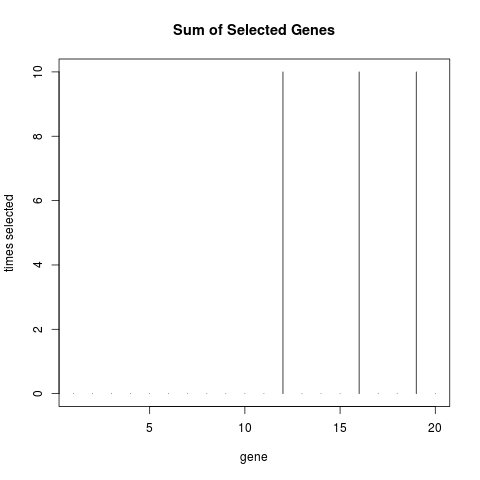
\includegraphics[width=\textwidth]{img/hist_small}
                \caption{Histogram}
                \label{fig:gull}
        \end{subfigure}%
        ~ %add desired spacing between images, e. g. ~, \quad, \qquad, \hfill etc.
          %(or a blank line to force the subfigure onto a new line)
        \begin{subfigure}[b]{0.5\textwidth}
                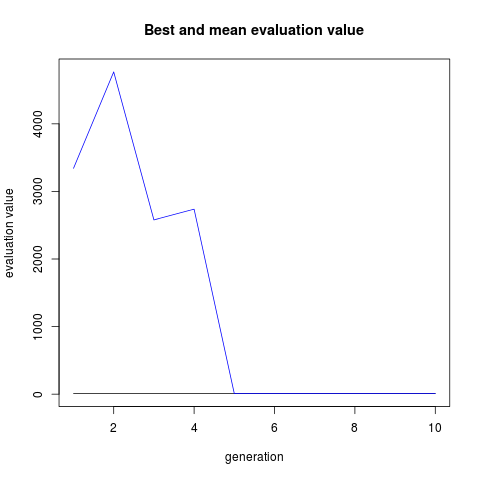
\includegraphics[width=\textwidth]{img/plot_small}
                \caption{Wynik funkcji ewaluacji}
                \label{fig:tiger}
        \end{subfigure}
        \caption{Wyniki dla konfiguracji \ref{small}}
        \label{fig:small}
\end{figure}

\begin{figure}[H]
        \centering
        \begin{subfigure}[b]{0.5\textwidth}
                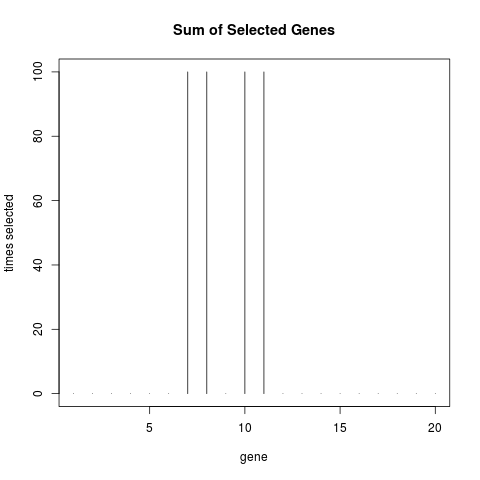
\includegraphics[width=\textwidth]{img/hist}
                \caption{Histogram}
                \label{fig:gull}
        \end{subfigure}%
        ~ %add desired spacing between images, e. g. ~, \quad, \qquad, \hfill etc.
          %(or a blank line to force the subfigure onto a new line)
        \begin{subfigure}[b]{0.5\textwidth}
                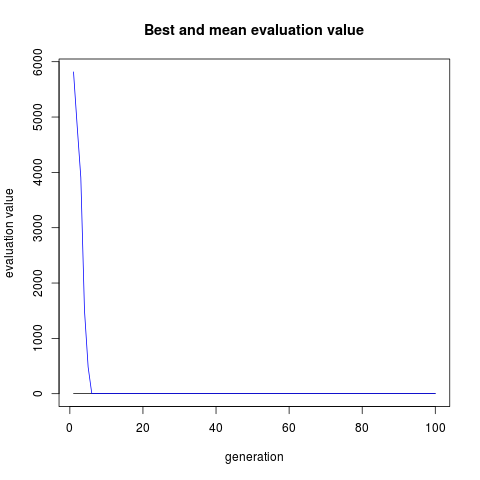
\includegraphics[width=\textwidth]{img/plot}
                \caption{Wynik funkcji ewaluacji}
                \label{fig:tiger}
        \end{subfigure}
        \caption{Wyniki dla konfiguracji \ref{mid}}
        \label{fig:small}
\end{figure}

\begin{figure}[H]
        \centering
        \begin{subfigure}[b]{0.5\textwidth}
                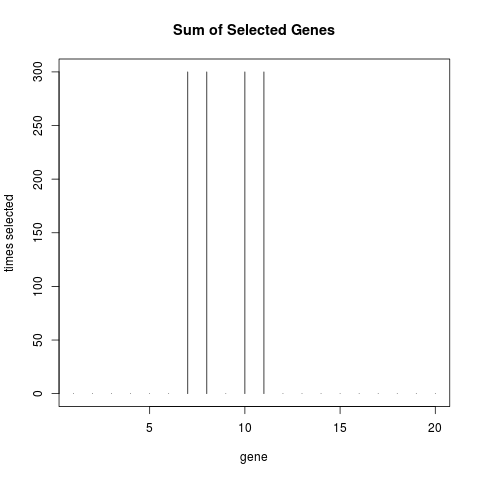
\includegraphics[width=\textwidth]{img/hist_big}
                \caption{Histogram}
                \label{fig:gull}
        \end{subfigure}%
        ~ %add desired spacing between images, e. g. ~, \quad, \qquad, \hfill etc.
          %(or a blank line to force the subfigure onto a new line)
        \begin{subfigure}[b]{0.5\textwidth}
                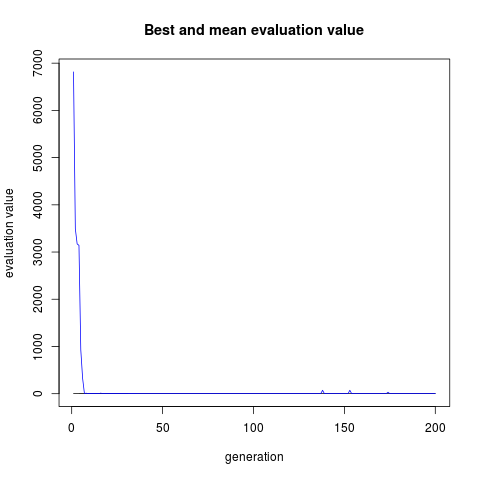
\includegraphics[width=\textwidth]{img/plot_big}
                \caption{Wynik funkcji ewaluacji}
                \label{fig:tiger}
        \end{subfigure}
        \caption{Wyniki dla konfiguracji \ref{big}}
        \label{fig:small}
\end{figure}

Niespodziewanie algorytm bardzo szybko zbiega do stabilnego rozwiązania przy dość małej
generacji początkowej. Nie zaobserwowano ochyleń. Wyłoniona konfiguracja to 
\begin{table}[H]
\caption{Najlepszy osobnik}
\label{the_choosen_one}
\centering
\begin{tabular}{|c|c|}
  Activation function                  & tanh \\
  Hidden Layer Size       & 216 \\ 
  Denominator & 1 \\
  Linear Output               & TRUE \\
\end{tabular} 
\end{table}

\subsection{Wnioski}
Dosyć duży rozmiar warstwy ukrytej pozwala sądzić, że algorytm dobrał
maksymalny możliwy rozmiar który daje się nauczyć przy ograniczonej liczbie 
iteracji. Perceptron zamiast uogólniać wiedzę stara się nauczyć każdego przypadku
oddzielnie. Prawdopodobnie przy zwiększeniu dopuszczalnej liczby iteracji
liczba neuronów warstwy ukrytej również by wzrosła.

W dalszych badaniach funkcja oceny powinna zostać rozszerzona o czynnik
przeciwdziałający nadmiernemu wzrostowi sieci (np. obecnie stosowana funkcja
mogła by być mnożona przez liczbę neuronów).

Inne prace wykazały małą przydatność perceptronów w problemie gry w \emph{connect4}.


%
% ---- Bibliography ----
%
\begin{thebibliography}{4}
%
\bibitem {arabas}
Arabas J.:
\textsl{Wykłady z algorytmów ewolucyjnych}, WNT Warszawa,2001
\bibitem {mandziuk2011}
Mandziuk, J.:
\textsl{Towards Cognitively Plausible Game Playing Systems}
IEEE COMPUTATIONAL INTELLIGENCE MAGAZINE, Maj, 2011
\bibitem {connect4:wiki}
\textsl{Connect Four --- {W}ikipedia{,} The Free Encyclopedia}
\url{http://en.wikipedia.org/wiki/Connect_Four}
\bibitem {velena}
\textsl{A Shannon C-type program which plays connect four perfectly}
\url{http://www.ce.unipr.it/~gbe/velena.html}
\bibitem{Riedmiller93adirect}
Martin Riedmiller and Heinrich Braun,
\textsl{A Direct Adaptive Method for Faster Backpropagation Learning: The RPROP Algorithm}
IEEE INTERNATIONAL CONFERENCE ON NEURAL NETWORKS, 1993,586--591
\bibitem{R:genalg}
\url{https://github.com/egonw/genalg}
\bibitem{R:neuralnet}
\url{http://cran.r-project.org/web/packages/neuralnet/}
\bibitem{R:cache}
Bengtsson, H. The R.oo package
\textsl{Object-Oriented Programming with References Using}
Standard R Code, Proceedings of the 3rd International Workshop on Distributed
Statistical Computing (DSC 2003), ISSN 1609-395X, Hornik, K.; Leisch, F. \& Zeileis,
A. (ed.), 2003
\end{thebibliography}

\end{document}
